% SIAM Article Template
\documentclass[r]{siamart171218}
% Packages and macros go here
\usepackage[english]{babel}
\usepackage{fullpage}
\usepackage{amsmath}
\usepackage{amssymb}
\usepackage{amsfonts}
\usepackage{array}
\usepackage{graphicx}
\usepackage{epsfig}
\usepackage{float}
\usepackage{fullpage}
\usepackage{color}
\usepackage{enumitem}  
\usepackage{epstopdf}
\usepackage{tikz}

% Title. If the supplement option is on, then "Supplementary Material"
% is automatically inserted before the title.
%\title{On the weak coupling of 3D and 1D second order elliptic problems}
\title{Coupling PDEs on XD-YD domains with Lagrange multipliers}

% Authors: full names plus addresses.
\author{
Miroslav Kuchta, Federica Laurino, Kent-Andre Mardal, Paolo Zunino,\thanks{Authors are listed in alphabetical order}
}

\begin{document}

\maketitle

% REQUIRED
\begin{abstract}
  This note summarizes numerical experiments investigating stabilization
  techniques for coupled multiscale problems using Lagrange multipliers.
  These are personal notes written to keep track of the developments on this
  topic, to be kept confidential.
\end{abstract}

% REQUIRED
\begin{keywords}
elliptic problems, high dimensionality gap, essential coupling conditions, Lagrange multipliers
\end{keywords}

% REQUIRED
\begin{AMS}
n.a.
\end{AMS}

% >>>>>>>>>>>>>>>>>>>>>>>>>>>>>>>>>>>>>>>>>>>>>>>>>>>>>>>>>>>>>>>>>>>>>>>>>>>>>>>>>>>>>>>>>>>>>>>>>>>>
 
\newcommand{\semi}[1]{\lvert{#1}\rvert}
\newcommand{\norm}[1]{\lVert{#1}\rVert}
\newcommand{\jump}[1]{\ensuremath{[\![#1]\!]} }
\newcommand{\avg}[1]{\ensuremath{\left\{\!\left\{#1\right\}\!\right\}} }


\newtheorem{thm}{Theorem}[section]
\newtheorem{prop}{Property}[section]
\theoremstyle{remark}
\newtheorem{remark}{Remark}[section]
 

\section{Babu{\v s}ka problem}\label{sec:babuska}
Given bounded $\Omega\subset\mathbb{R}^2$, let $\Gamma_D$, $\Gamma_L \subset \partial \Omega$ be such that $\semi{\Gamma_i}\neq 0$,
$i\in\left\{D, L\right\}$, $\bigcup_{i}\Gamma_i=\partial\Omega$.
We then consider the Poisson problem 
\[
\begin{aligned}
-\Delta u &= f &\mbox{ in }\Omega,\\
u &= g &\mbox{ on }\Gamma_D,\\
u &= g &\mbox{ on }\Gamma_L,\\
\end{aligned}
\]
which upon introducing the Lagrange multiplier $p\in Q=(H^{1/2}_{00}(\Gamma_L))^{\prime}$
leads to a variational problem: Find $u\in V=H^1_{0, \Gamma_D}(\Omega)$,
$p\in Q$ such that
%
\begin{equation}\label{eq:bab}
  \begin{aligned}
    &\int_{\Omega} \nabla u\cdot \nabla v &+ \int_{\Gamma_L}p v &= \int_{\Omega} f v &\forall v\in V,\\
    &\int_{\Gamma_L}q u  &\phantom{+\int_{\Omega} \nabla u\cdot \nabla v} &= \int_{\Gamma} g q &\forall q\in Q.
  \end{aligned}
\end{equation}
%

In the following experiments $\Omega=(0, 1)^2$, $\Gamma_L=\left\{(x, y)\in\partial\Omega; x=0\right\}$
while $\Gamma_D=\partial\Omega\setminus \Gamma_L$. Letting $\Omega_H$, $\Gamma_h$
denote respectively the discretizations of $\Omega$ and $\Gamma_L$ we shall consider
two different geometrical settings, cf. Figure \ref{fig:domains}, (i) either
$\Gamma_h$ is the trace mesh (on $\Gamma_L$) of $\Omega$, i.e. there is a one-to-one
mapping between vertices/cells of the two meshes or (ii) $\Gamma_h$ is not the
trace mesh of $\Omega$ and $\Gamma_h$ is finer relative to the trace mesh.
We shall subsequently refer to the two cases as \emph{matching} and \emph{non-matching}.

%
\begin{figure}[h]
  \begin{center}
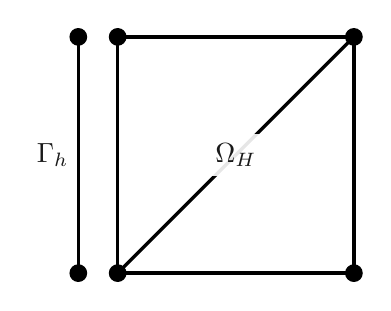
\begin{tikzpicture}
  \draw[black, very thick] (1,0) rectangle (4, 3);
  \draw[black, very thick] (1,0) -- (4, 3);
  \node[fill=white, opacity=0.9] at (2.5, 1.5) {$\Omega_{H}$};

  \node[mark size=3pt, color=black] at (1, 0) {\pgfuseplotmark{*}};
  \node[mark size=3pt, color=black] at (4, 0) {\pgfuseplotmark{*}};
  \node[mark size=3pt, color=black] at (1, 3) {\pgfuseplotmark{*}};
  \node[mark size=3pt, color=black] at (4, 3) {\pgfuseplotmark{*}};

  \draw[black, very thick] (0.5,0) -- (0.5, 3);
  \node[opacity=0.9, left] at (0.5, 1.5) {$\Gamma_{h}$};

  \node[mark size=3pt, color=black] at (0.5, 0) {\pgfuseplotmark{*}};
  \node[mark size=3pt, color=black] at (0.5, 3) {\pgfuseplotmark{*}};
\end{tikzpicture}
%
\hspace{50pt}
%
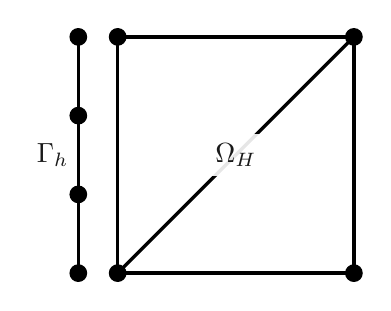
\begin{tikzpicture}
  \draw[black, very thick] (1,0) rectangle (4, 3);
  \draw[black, very thick] (1,0) -- (4, 3);
  \node[fill=white, opacity=0.9] at (2.5, 1.5) {$\Omega_{H}$};

  \node[mark size=3pt, color=black] at (1, 0) {\pgfuseplotmark{*}};
  \node[mark size=3pt, color=black] at (4, 0) {\pgfuseplotmark{*}};
  \node[mark size=3pt, color=black] at (1, 3) {\pgfuseplotmark{*}};
  \node[mark size=3pt, color=black] at (4, 3) {\pgfuseplotmark{*}};

  \draw[black, very thick] (0.5,0) -- (0.5, 3);
  \node[opacity=0.9, left] at (0.5, 1.5) {$\Gamma_{h}$};

  \node[mark size=3pt, color=black] at (0.5, 0) {\pgfuseplotmark{*}};
  \node[mark size=3pt, color=black] at (0.5, 1) {\pgfuseplotmark{*}};
  \node[mark size=3pt, color=black] at (0.5, 2) {\pgfuseplotmark{*}};  
  \node[mark size=3pt, color=black] at (0.5, 3) {\pgfuseplotmark{*}};
\end{tikzpicture}
%
\end{center}
  \caption{Matching (left) and non-mathching (right) setting considered
    for the Babu{\v s}ka problem.}
\label{fig:domains}
\end{figure}


\subsection{Discretization by P1-P1 elements}\label{sec:p1_p1} We consider
finite element discretization of \eqref{eq:bab} in terms continuous linear
Lagrange elements (P1) for both spaces $V$ and $Q$.

\subsubsection{Matching case} We remark that Dirichlet boundary conditions
$p=0$ on $\partial\Gamma_L$ need to be enforced on the linear system in order
to obtain a non-singular system matrix. Then the discretization is inf-sup
stable as can be seen in Table \ref{tab:p1_p1} by observing that the MinRes
iterations using the Riesz map preconditioner remain bounded in the discretization
parameter. Note that the $Q$ block of (the diagonal) preconditioner represents
the action of the inverse of $-\Delta^{1/2}_{00}$. In particular, the fractional
operator is based on the eigenvalue problem
%
\[
\begin{aligned}
  -\Delta p &= \lambda p &\mbox{ in }\Gamma_L,\\
          p &= 0         &\mbox{ on }\partial\Gamma_L.
\end{aligned}
\]
%

\subsubsection{Non-matching case} Here $\dim Q_h$ is (considerably) larger
than the trace space of $V_H$ and stabilization of \cite{burman2009interior}
is needed to obtain inf-sup stability. More precisely, the discretization
of \eqref{eq:bab} reads: Find $u\in V_H$, $q\in Q_h$ such that
%
\begin{equation}\label{eq:p1_stab}
\begin{aligned}
&\int_{\Omega} \nabla u\cdot \nabla v &+ \int_{\Gamma_L}p v &= \int_{\Omega} f v &\forall v\in V_H,\\
  &\int_{\Gamma_L}q u  &-\gamma \sum_{K\in\Gamma_h}\int_{K} h_K^3\nabla p\cdot\nabla q &= \int_{\Gamma} g q &\forall q\in Q_h.
  \end{aligned}
\end{equation}
%
Here $\gamma$ is a stabilization parameter and we use $\gamma=1$ in the
following. As before, the trial and test functions of the space $Q_h$ are
constructed such that they satisfy the boundary conditions $p=0$ on $\partial\Gamma_L$.

MinRes iteration counts with the Riesz map preconditioner are shown in
Table \ref{tab:p1_p1}. Here, the $Q$ block of the preconditioner is based
on the inverse of the bilinear form
\[
\langle -\Delta_{00}^{1/2} p, q\rangle + \sum_{K\in\Gamma_h}\int_{K} h_K^3\nabla p \cdot\nabla q,\quad p, q\in Q_h.
\]
%

\begin{table}
  \begin{center}
    \footnotesize{
  \begin{tabular}{c|cc|c|c||cc|c|c}
    \hline
    $h$ & $\norm{u-u_H}_1$ & $\norm{p-p_h}_0$ & $n$ & $\kappa$
        & $\norm{u-u_H}_1$ & $\norm{p-p_h}_0$ & $n$ & $\kappa$ \\
    \hline
8.84E-02 & 6.91E+00(--)   & 6.37E+00(--)   & 29 & 5.131 & 6.90E+00(--)  & 5.94E+00(--)    & 31 & 4.836\\
4.42E-02 & 3.54E+00(0.97) & 1.61E+00(1.98) & 26 & 5.176 & 3.54E+00(0.96) & 1.76E+00(1.75) & 29 & 4.846\\
2.21E-02 & 1.78E+00(0.99) & 5.45E-01(1.56) & 26 & 5.191 & 1.78E+00(0.99) & 5.95E-01(1.57) & 28 & 4.851\\
1.10E-02 & 8.93E-01(1.00) & 3.11E-01(0.81) & 25 & 5.195 & 8.93E-01(1.00) & 3.24E-01(0.88) & 26 & 4.853\\
5.52E-03 & 4.46E-01(1.00) & 2.12E-01(0.55) & 24 & 5.196 & 4.46E-01(1.00) & 2.16E-01(0.59) & 26 & 4.853\\
2.76E-03 & 2.23E-01(1.00) & 1.49E-01(0.51) & 24 & 5.196 & 2.23E-01(1.00) & 1.50E-01(0.52) & 24 & 4.854\\
1.38E-03 & 1.12E-01(1.00) & 1.06E-01(0.50) & 22 & --    & 1.12E-01(1.00) & 1.06E-01(0.51) & 22 & --   \\
    \hline
  \end{tabular}
  }
    \caption{Approximation errors, number of preconditioned MinRes iterations ($n$) and
      condition number of the preconditioned problem \eqref{eq:bab} ($\kappa$) discretized
      with P1-P1 elements. (left) Matching case. (right) Non-matching case.}
  \label{tab:p1_p1}
  \end{center}
\end{table}
%
Concerning approximation properties of the discretization, note that the error
for the multiplier is reported in the $L^2$ norm and not the natural $H^{-1/2}$
norm. Nevertheless, the rate seems sub-optimal. This is likely due to the fact
that the multiplier in the manufactured test case does not satisfy the
Dirichlet boundary conditions employed in the discrete problem.

\subsection{Discretization by P1-P0 elements}\label{sec:p1_p0}
We consider finite element discretization of \eqref{eq:bab} in terms P1 elements
for the space $V$ while the multiplier space uses piecewise constants elements
(P0). In both the matching and non-matching case the discretization is unstable
and inf-sup stability is obtained by using stabilization \cite{burman2014projection}.
That is, the disretization of \eqref{eq:bab} reads: Find $u\in V_H$, $q\in Q_h$ such that
%
\begin{equation}\label{eq:p0_stab}
\begin{aligned}
&\int_{\Omega} \nabla u\cdot \nabla v &+ \int_{\Gamma_L}p v &= \int_{\Omega} f v &\forall v\in V_H,\\
  &\int_{\Gamma_L}q u  &-\gamma \sum_{\mathcal{V}^0} \avg{h_K}^2\jump{p}\jump{q} &= \int_{\Gamma} g q &\forall q\in Q_h,
  \end{aligned}
\end{equation}
%
where $\mathcal{V}^0$ is the set of all interior vertices of $\Gamma_h$.

Table \ref{tab:p1_p0} shows stability and convergence properties of the approximation.
Note that the error in the multiplier converges linearly, cf. $\tfrac{1}{2}$ for
the P1-P1 discretization in Table \ref{tab:p1_p1}.

\begin{table}
  \begin{center}
    \footnotesize{
  \begin{tabular}{c|cc|c|c||cc|c|c}
    \hline
    $h$ & $\norm{u-u_H}_1$ & $\norm{p-p_h}_0$ & $n$ & $\kappa$
        & $\norm{u-u_H}_1$ & $\norm{p-p_h}_0$ & $n$ & $\kappa$ \\
    \hline
8.84E-02 & 6.88E+00(--)   & 2.83E+00(--)  & 26 & 4.749  & 6.91E+00(--)   & 1.17E+01(--)  & 35 & 6.940 \\
4.42E-02 & 3.54E+00(0.96) & 2.12E+00(0.42)& 28 & 4.817  & 3.54E+00(0.96) & 2.33E+00(2.33)& 35 & 6.973 \\
2.21E-02 & 1.78E+00(0.99) & 7.42E-01(1.51)& 28 & 4.840  & 1.78E+00(0.99) & 4.91E-01(2.24)& 30 & 6.987 \\
1.10E-02 & 8.93E-01(1.00) & 2.17E-01(1.78)& 25 & 4.850  & 8.93E-01(1.00) & 1.46E-01(1.75)& 28 & 6.994 \\
5.52E-03 & 4.46E-01(1.00) & 8.90E-02(1.28)& 23 & 4.853  & 4.46E-01(1.00) & 5.90E-02(1.31)& 27 & 6.996 \\
2.76E-03 & 2.23E-01(1.00) & 4.28E-02(1.06)& 23 & 4.853  & 2.23E-01(1.00) & 2.77E-02(1.09)& 26 & 6.995 \\
1.38E-03 & 1.12E-01(1.00) & 2.12E-02(1.01)& 23 & --     & 1.12E-01(1.00) & 1.36E-02(1.02)& 25 & --    \\  
    \hline
  \end{tabular}
    }
    \caption{Approximation errors, number of preconditioned MinRes iterations ($n$) and
      condition number of the preconditioned problem \eqref{eq:bab} ($\kappa$) discretized
      with P1-P0 elements. (left) Matching case. (right) Non-matching case.}
  \label{tab:p1_p0}
  \end{center}
\end{table}

\section{Coupled multiscale problem}\label{sec:coupled} As a stepping stone
towards the coupled 3$d$-1$d$-1$d$ problem we consider first a coupled multiscale
problem where the dimensionality gap is 1. Given two bounded domains $\Omega^i \subset\mathbb{R}^2$,
$i\in\left\{-, +\right\}$, let $\Gamma$ be the intersection of the domain boundaries,
cf. Figure \ref{fig:coupled_domain}. We are then interested in solving

\begin{minipage}{0.47\textwidth}
  \begin{equation}\label{eq:coupled}
    \begin{aligned}
      -\Delta u^i &= f &\mbox{ in }\Omega^{i}, i\in\left\{+, -\right\},\\
      u^i &= g^i &\mbox{ on }\Gamma^i_D=\partial\Omega^{i}\setminus\Gamma,\\
      \jump{u} &= 0 &\mbox{ on }\Gamma,\\
      -\Delta \hat{u} - \jump{\nabla u\cdot n}&= \hat{f} &\mbox{ on }\Gamma,\\
      \hat{u} &= \hat{g} &\mbox{ on }\partial\Gamma,\\
      u - \hat{u} &= h&\mbox{ on }\Gamma.\\
    \end{aligned}
\end{equation}
\null
\par\xdef\tpd{\the\prevdepth}
\end{minipage}
\hfill
\begin{minipage}{0.47\textwidth}
  \begin{figure}[H]
    \begin{center}
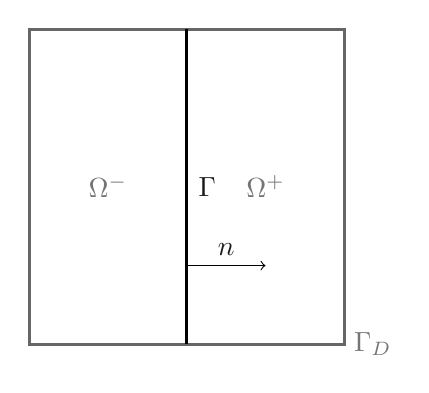
\begin{tikzpicture}
  \draw[black!60!white, very thick] (0,0) rectangle (4, 4);
  \draw[black!60!white, very thick] (2, 0) rectangle (2, 4);

  \node[black!60!white, fill=white, opacity=0.9] at (1, 2) {$\Omega^{-}$};
  \node[black!60!white, fill=white, opacity=0.9] at (3, 2) {$\Omega^{+}$};
  \node[black!60!white, opacity=0.9, right] at (4, 0) {$\Gamma_D$};
  
  \draw[black, very thick] (2, 0) -- (2, 4);
  \draw[->, black] (2, 1) -- (3, 1);
  \node[fill=white, opacity=0.9, above] at (2.5, 1) {$n$};
  \node[fill=white, opacity=0.9, right] at (2.025, 2) {$\Gamma$};
\end{tikzpicture}
    \end{center}
    %\vspace{-20pt}
    \caption{Schematic domain of coupled multiscale problem.}
    \label{fig:coupled_domain}
    %\vspace{5pt}    
\end{figure}
\end{minipage}
%
Let $\Omega=\Omega^{+}\cup\Omega^{-}$ and $\Gamma_D=\Gamma^{+}_D\cup\Gamma^{-}_N$.
Introducing a Lagrange multiplier $p=\jump{\nabla u \cdot n}\in Q=(H^{-1/2}_{00}(\Gamma))^{\prime}$
the weak form of \eqref{eq:coupled} reads: Find $u\in V=H^1_{0, \Gamma_D}(\Omega)$,
$\hat{v}\in\hat{V}=H^1_{0, \partial\Gamma}(\Gamma)$, $p\in Q$ such that
%
\begin{equation}\label{eq:coupled_weak}
  \begin{aligned}
    &\int_{\Omega}\nabla u\cdot \nabla v &\phantom{+\int_{\Gamma}\nabla \hat{u}\cdot \nabla \hat{v}} &+\int{\Gamma}p v &= \int_{\Omega}f v \quad &\forall v\in V,\\
    &\phantom{\int_{\Omega}\nabla u\cdot \nabla v} &+{\int_{\Gamma}\nabla \hat{u}\cdot \nabla \hat{v}} &-\int{\Gamma}p\hat{v} &= \int_{\Gamma}\hat{f}\hat{v} \quad &\forall \hat{v}\in \hat{V},\\
    &\int_{\Gamma}u q &-\int_{\Gamma}\hat{u}q &\phantom{-\int{\Gamma}q\hat{v}} &= \int_{\Gamma}h q \quad &\forall q\in Q.
  \end{aligned}
\end{equation}
%
\begin{figure}[h]
  \begin{center}
    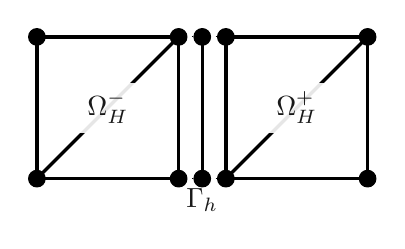
\begin{tikzpicture}[scale=0.60]
      % Minus
  \draw[black, very thick] (1,0) rectangle (4, 3);
  \draw[black, very thick] (1,0) -- (4, 3);
  \node[fill=white, opacity=0.9] at (2.5, 1.5) {$\Omega^{-}_{H}$};

  \node[mark size=3pt, color=black] at (1, 0) {\pgfuseplotmark{*}};
  \node[mark size=3pt, color=black] at (4, 0) {\pgfuseplotmark{*}};
  \node[mark size=3pt, color=black] at (1, 3) {\pgfuseplotmark{*}};
  \node[mark size=3pt, color=black] at (4, 3) {\pgfuseplotmark{*}};

  \draw[black, thin, dotted] (4, 0) -- (4.5, 0);
  \draw[black, thin, dotted] (4, 3) -- (4.5, 3);
  % Center
  \draw[black, thin, dotted] (4.5, 0) -- (5, 0);
  \draw[black, thin, dotted] (4.5, 3) -- (5, 3);
  
  \draw[black, very thick] (4.5,0) -- (4.5, 3);
  \node[opacity=0.9, below] at (4.5, 0) {$\Gamma_{h}$};

  \node[mark size=3pt, color=black] at (4.5, 0) {\pgfuseplotmark{*}};
  \node[mark size=3pt, color=black] at (4.5, 3) {\pgfuseplotmark{*}};
  % Right
    \draw[black, very thick] (5,0) rectangle (8, 3);
  \draw[black, very thick] (5,0) -- (8, 3);
  \node[fill=white, opacity=0.9] at (6.5, 1.5) {$\Omega^{+}_{H}$};

  \node[mark size=3pt, color=black] at (5, 0) {\pgfuseplotmark{*}};
  \node[mark size=3pt, color=black] at (8, 0) {\pgfuseplotmark{*}};
  \node[mark size=3pt, color=black] at (5, 3) {\pgfuseplotmark{*}};
  \node[mark size=3pt, color=black] at (8, 3) {\pgfuseplotmark{*}};
\end{tikzpicture}
    %
    \hspace{10pt}
    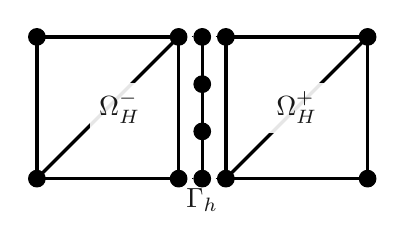
\begin{tikzpicture}[scale=0.60]
      % Minus
  \draw[black, very thick] (1,0) rectangle (4, 3);
  \draw[black, very thick] (1,0) -- (4, 3);
  \node[fill=white, opacity=0.9] at (2.75, 1.5) {$\Omega^{-}_{H}$};

  \node[mark size=3pt, color=black] at (1, 0) {\pgfuseplotmark{*}};
  \node[mark size=3pt, color=black] at (4, 0) {\pgfuseplotmark{*}};
  \node[mark size=3pt, color=black] at (1, 3) {\pgfuseplotmark{*}};
  \node[mark size=3pt, color=black] at (4, 3) {\pgfuseplotmark{*}};
  
  \draw[black, thin, dotted] (4, 0) -- (4.5, 0);
  \draw[black, thin, dotted] (4, 3) -- (4.5, 3);
  % Center
  \draw[black, thin, dotted] (4.5, 0) -- (5, 0);
  \draw[black, thin, dotted] (4.5, 3) -- (5, 3);
     % Center
  \draw[black, very thick] (4.5,0) -- (4.5, 3);
  \node[opacity=0.9, below] at (4.5, 0) {$\Gamma_{h}$};

  \node[mark size=3pt, color=black] at (4.5, 0) {\pgfuseplotmark{*}};
  \node[mark size=3pt, color=black] at (4.5, 1) {\pgfuseplotmark{*}};
  \node[mark size=3pt, color=black] at (4.5, 2) {\pgfuseplotmark{*}};
  \node[mark size=3pt, color=black] at (4.5, 3) {\pgfuseplotmark{*}};
  % Right
    \draw[black, very thick] (5,0) rectangle (8, 3);
  \draw[black, very thick] (5,0) -- (8, 3);
  \node[fill=white, opacity=0.9] at (6.5, 1.5) {$\Omega^{+}_{H}$};

  \node[mark size=3pt, color=black] at (5, 0) {\pgfuseplotmark{*}};
  \node[mark size=3pt, color=black] at (8, 0) {\pgfuseplotmark{*}};
  \node[mark size=3pt, color=black] at (5, 3) {\pgfuseplotmark{*}};
  \node[mark size=3pt, color=black] at (8, 3) {\pgfuseplotmark{*}};
    \end{tikzpicture}
        %
    \hspace{10pt}
    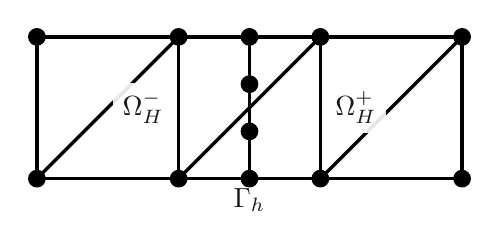
\begin{tikzpicture}[scale=0.60]
      % Minus
  \draw[black, very thick] (0,0) rectangle (3, 3);
  \draw[black, very thick] (0,0) -- (3, 3);
  \node[fill=white, opacity=0.9] at (2.25, 1.5) {$\Omega^{-}_{H}$};

  \node[mark size=3pt, color=black] at (0.0, 0) {\pgfuseplotmark{*}};
  \node[mark size=3pt, color=black] at (3.0, 0) {\pgfuseplotmark{*}};
  \node[mark size=3pt, color=black] at (0.0, 3) {\pgfuseplotmark{*}};
  \node[mark size=3pt, color=black] at (3.0, 3) {\pgfuseplotmark{*}};
  
     % Center
  \draw[black, very thick] (4.5,0) -- (4.5, 3);
  \node[opacity=0.9, below] at (4.5, 0) {$\Gamma_{h}$};

  \node[mark size=3pt, color=black] at (4.5, 0) {\pgfuseplotmark{*}};
  \node[mark size=3pt, color=black] at (4.5, 1) {\pgfuseplotmark{*}};
  \node[mark size=3pt, color=black] at (4.5, 2) {\pgfuseplotmark{*}};
  \node[mark size=3pt, color=black] at (4.5, 3) {\pgfuseplotmark{*}};

  \draw[black, very thick] (3,0) -- (6, 0);
  \draw[black, very thick] (3,0) -- (6, 3);
  \draw[black, very thick] (3,3) -- (6, 3);  
  % Right
    \draw[black, very thick] (6,0) rectangle (9, 3);
  \draw[black, very thick] (6,0) -- (9, 3);
  \node[fill=white, opacity=0.9] at (6.75, 1.5) {$\Omega^{+}_{H}$};

  \node[mark size=3pt, color=black] at (6, 0) {\pgfuseplotmark{*}};
  \node[mark size=3pt, color=black] at (9, 0) {\pgfuseplotmark{*}};
  \node[mark size=3pt, color=black] at (6, 3) {\pgfuseplotmark{*}};
  \node[mark size=3pt, color=black] at (9, 3) {\pgfuseplotmark{*}};
\end{tikzpicture}
%
\end{center}
  \caption{Different mesh settings considered for the coupled problem
    \eqref{eq:coupled_weak}: conforming matching, conforming non-matching,
    non-conforming (from left to right).
  }
\label{fig:multi_domains}
\end{figure}
%
In the following $\Omega=(0, 1)$, $\Gamma=\left\{(x, y)\in\Omega; x=\tfrac{1}{2}\right\}$
and based on the properties of the finite element meshes $\Omega_H$, $\Gamma_h$
we shall distinguish three different settings, cf. Figure \ref{fig:multi_domains}.
Here, a conforming case implies that the trace mesh of $\Omega_H$ on $\Gamma$
consists only of the existing facets of the mesh. In the conforming setting 
we consider matching and non-matching cases as defined above. We remark
that the approximation of the space $\hat{V}$ shall always be constructed
on the multiplier mesh $\Gamma_h$.

\subsection{P1-P1-P1 discretization with $\Gamma$ conformity}
Let us first consider a conforming setting and an approximation of all
the spaces involved in \eqref{eq:coupled_weak} in terms of P1 elements.
As with the Babu{\v s}ka problem \eqref{eq:bab} the discrete multiplier
space is such that $q=0$ on $\partial\Gamma$ for all $q\in Q_h$. In fact,
the boundary conditions are necessary to obtain an invertible linear system.

Table \ref{tab:coupled_p1_p1} summarizes the results for both matching
and non-matching tessilations. In the latter case, a stabilization term
\cite{burman2009interior} is added similar to \eqref{eq:p1_stab} (we set $\gamma=1$).
In both cases the results show evidence of the inf-sup stability of the
discretization. We note that the $L^2$ error of the multiplier converges
quadratically; in contrast to the test problem in \eqref{eq:bab} the solution
here \emph{does} satisfy $p=0$ on $\partial\Gamma$.

\begin{table}
  \begin{center}
    \scriptsize{
  \begin{tabular}{c|ccc|c|c||ccc|c|c}
    \hline
    $h$ & $\norm{u-u_H}_1$ & $\norm{\hat{u}-\hat{u}_h}_1$ & $\norm{p-p_h}_0$ & $n$ & $\kappa$
        & $\norm{u-u_H}_1$ & $\norm{\hat{u}-\hat{u}_h}_1$ & $\norm{p-p_h}_0$ & $n$ & $\kappa$ \\
    \hline
8.8E-2 & 8.8E-1(--)   & 2.0E0(--)    & 8.9E-1(--)   & 20 & 8.0 & 8.6E-1(--)   & 6.7E-1(--)   & 1.7E-1(--)   & 23 & 4.5  \\
4.4E-2 & 4.4E-1(1.01) & 1.0E0(0.99)  & 2.1E-1(2.10) & 22 & 8.4 & 4.4E-1(0.99) & 3.4E-1(1.00) & 4.5E-2(1.89) & 25 & 4.5  \\
2.2E-2 & 2.2E-1(1.00) & 5.0E-1(1.00) & 5.1E-2(2.03) & 22 & 8.5 & 2.2E-1(1.00) & 1.7E-1(1.00) & 1.2E-2(1.95) & 25 & 4.6  \\
1.1E-2 & 1.1E-1(1.00) & 2.5E-1(1.00) & 1.3E-2(2.01) & 21 & 8.6 & 1.1E-1(1.00) & 8.4E-2(1.00) & 3.0E-3(1.98) & 24 & 4.7  \\
5.5E-3 & 5.5E-2(1.00) & 1.3E-1(1.00) & 3.2E-3(2.00) & 21 & 8.7 & 5.5E-2(1.00) & 4.2E-2(1.00) & 7.5E-4(1.99) & 24 & 4.7  \\
2.8E-3 & 2.7E-2(1.00) & 6.3E-2(1.00) & 7.9E-4(2.00) & 21 & 8.7 & 2.7E-2(1.00) & 2.1E-2(1.00) & 1.9E-4(1.99) & 22 & 4.7  \\
1.4E-3 & 1.4E-2(1.00) & 3.1E-2(1.00) & 2.0E-4(2.00) & 21 & --  & 1.4E-2(1.00) & 1.0E-2(1.00) & 4.7E-5(2.00) & 22 & --   \\
    \hline
  \end{tabular}
    }
    \caption{Approximation errors, number of preconditioned MinRes iterations ($n$) and
      condition number of the preconditioned problem \eqref{eq:coupled_weak} ($\kappa$) discretized
      with P1-P1-P1 elements. Conforming (left) matching and (right) non-matching case.}
  \label{tab:coupled_p1_p1}
  \end{center}
\end{table}

% --------------------------------------------------------------------

\subsection{P1-P1-P0 discretization with $\Gamma$ conformity} 
We shall next have the multiplier space be spanned by piecewise constant
functions. Following \eqref{eq:bab} a stabilization \cite{burman2014projection}
is employed in both the matching and non-matching cases. Table \ref{tab:coupled_p1_p0}
confirms that the discretization is inf-sup stable. 

\begin{table}
  \begin{center}
    \scriptsize{
  \begin{tabular}{c|ccc|c|c||ccc|c|c}
    \hline
    $h$ & $\norm{u-u_h}_1$ & $\norm{\hat{u}-\hat{u}_h}_1$ & $\norm{p-p_h}_0$ & $n$ & $\kappa$
        & $\norm{u-u_h}_1$ & $\norm{\hat{u}-\hat{u}_h}_1$ & $\norm{p-p_h}_0$ & $n$ & $\kappa$ \\
    \hline
8.8E-2 & 9.3E-1(--)   & 2.0E0(--)    & 2.9E0(--)    & 21 & 4.5 & 8.6E-1(--)   & 6.7E-1(--)   & 9.2E-1(--)   & 29 & 7.8\\
4.4E-2 & 4.4E-1(1.06) & 1.0E0(0.99)  & 1.1E0(1.43)  & 28 & 4.8 & 4.4E-1(0.99) & 3.4E-1(1.00) & 3.4E-1(1.42) & 31 & 8.1\\
2.2E-2 & 2.2E-1(1.02) & 5.0E-1(1.00) & 4.1E-1(1.39) & 28 & 5.0 & 2.2E-1(1.00) & 1.7E-1(1.00) & 1.4E-1(1.34) & 32 & 8.3\\
1.1E-2 & 1.1E-1(1.00) & 2.5E-1(1.00) & 1.7E-1(1.28) & 27 & 5.1 & 1.1E-1(1.00) & 8.4E-2(1.00) & 5.6E-2(1.26) & 30 & 8.4\\
5.5E-3 & 5.5E-2(1.00) & 1.3E-1(1.00) & 7.5E-2(1.19) & 27 & 5.2 & 5.5E-2(1.00) & 4.2E-2(1.00) & 2.5E-2(1.18) & 30 & 8.5\\
2.8E-3 & 2.7E-2(1.00) & 6.3E-2(1.00) & 3.5E-2(1.11) & 27 & 5.2 & 2.7E-2(1.00) & 2.1E-2(1.00) & 1.1E-2(1.11) & 29 & 8.5\\
1.4E-3 & 1.4E-2(1.00) & 3.1E-2(1.00) & 1.7E-2(1.07) & 27 & --  & 1.4E-2(1.00) & 1.0E-2(1.00) & 5.5E-3(1.06) & 29 & -- \\
    \hline
  \end{tabular}
    }
    \caption{Approximation errors, number of preconditioned MinRes iterations ($n$) and
      condition number of the preconditioned problem \eqref{eq:coupled_weak} ($\kappa$) discretized
      with P1-P1-P0 elements. Conforming (left) matching and (right) non-matching case.}
  \label{tab:coupled_p1_p0}
  \end{center}
\end{table}

% -------------------------------------------------------------------

\subsection{Non-conforming setting}
Finally a non-conforming setting is considered with P1-P1-P1 and P1-P1-P0
discretizations. In both cases stabilization terms are employed to obtain
inf-sup stability, cf. Table \ref{tab:coupled_non}. Note that compared to the
conforming case the multiplier convergence with P1 elements is only linear.
The order from the conforming case is preserved with P0 elements. Note also
that with both elements $u_h$ converges with order $\tfrac{1}{2}$; the approximation
struggles to capture the kink of the solution which now occurs within the finite element
cells.

\begin{table}
  \begin{center}
    \scriptsize{
  \begin{tabular}{c|ccc|c|c||ccc|c|c}
    \hline
    $h$ & $\norm{u-u_H}_1$ & $\norm{\hat{u}-\hat{u}_h}_1$ & $\norm{p-p_h}_0$ & $n$ & $\kappa$
        & $\norm{u-u_H}_1$ & $\norm{\hat{u}-\hat{u}_h}_1$ & $\norm{p-p_h}_0$ & $n$ & $\kappa$ \\
    \hline
8.3E-2 & 1.3E0(--)    & 7.0E-1(--)   & 1.2E0(--)    & 28 & 5.2 & 1.3E0(--)    & 7.0E-1(--)   & 1.7E0(--)     & 31 & 8.6\\   
4.3E-2 & 8.1E-1(0.68) & 3.5E-1(1.04) & 6.4E-1(0.95) & 29 & 5.6 & 8.1E-1(0.68) & 3.5E-1(1.04) & 7.6E-1(1.18)  & 34 & 9.3\\ 
2.2E-2 & 5.3E-1(0.62) & 1.8E-1(1.02) & 3.3E-1(0.99) & 29 & 5.8 & 5.3E-1(0.62) & 1.8E-1(1.02) & 3.6E-1(1.10)  & 34 & 9.7\\ 
1.1E-2 & 3.6E-1(0.57) & 8.8E-2(1.01) & 1.6E-1(1.00) & 27 & 6.0 & 3.6E-1(0.57) & 8.8E-2(1.01) & 1.8E-1(1.05)  & 34 & 9.9\\ 
5.5E-3 & 2.5E-1(0.54) & 4.4E-2(1.01) & 8.3E-2(1.00) & 27 & 6.0 & 2.5E-1(0.54) & 4.4E-2(1.01) & 8.7E-2(1.03)  & 33 & 10.0\\
2.8E-3 & 1.7E-1(0.52) & 2.2E-2(1.00) & 4.1E-2(1.00) & 26 & 6.1 & 1.7E-1(0.52) & 2.2E-2(1.00) & 4.3E-2(1.01)  & 32 & 10.0\\
1.4E-3 & 1.2E-1(0.51) & 1.1E-2(1.00) & 2.1E-2(1.00) & 26 & --  & 1.2E-1(0.51) & 1.1E-2(1.00) & 2.1E-2(1.01)  & 31 & 10.0\\
    \hline
  \end{tabular}
    }
    \caption{Non-conforming setting. Approximation errors, number of preconditioned MinRes iterations ($n$) and
      condition number of the preconditioned problem \eqref{eq:coupled_weak} ($\kappa$) discretized
      with P1-P1-P1 (left) and P1-P1-P0 (right) elements.}
  \label{tab:coupled_non}
  \end{center}
\end{table}


\bibliographystyle{siamplain}
\bibliography{stab}
\end{document}
